\documentclass[10pt,aspectratio=149]{beamer}
\usecolortheme{Calm}
\usetheme{Calm}
\usepackage{pgfplots}
\usepackage{pgfplotstable}
\usepackage[utf8]{inputenc}
\usepackage{hyperref}
\RequirePackage[absolute,overlay]{textpos}
%\usepackage[sfdefault]{cabin}
%\usepackage[T1]{fontenc}
%\setlength{\TPHo{}rizModule}{\paperwidth}
%\setlength{\TPVertModule}{\paperheight}
%\definecolor{OQEdarkblue}{HTML}{046085}


\defbeamertemplate*{background canvas}{bg}
{%
  \color{lightgray!40}\vrule width\paperwidth height\paperheight% added bg color
}

%------------------------------

\author{Dominique Gravel}
\title{A brief history of spatial ecology}
\date{August 24th, 2026}
\institute{Université de Sherbrooke \\ Summer school in biodiversity modelling}

%------------------------------
% TITLE SLIDE
%------------------------------

\usebackgroundtemplate
{
  
\includegraphics[width=\paperwidth,height=\paperheight]{bg}%
}

\begin{document}

	\begin{frame}[plain]
		\titlepage
	\end{frame}

%------------------------------

\begin{frame}

    \begin{center}
        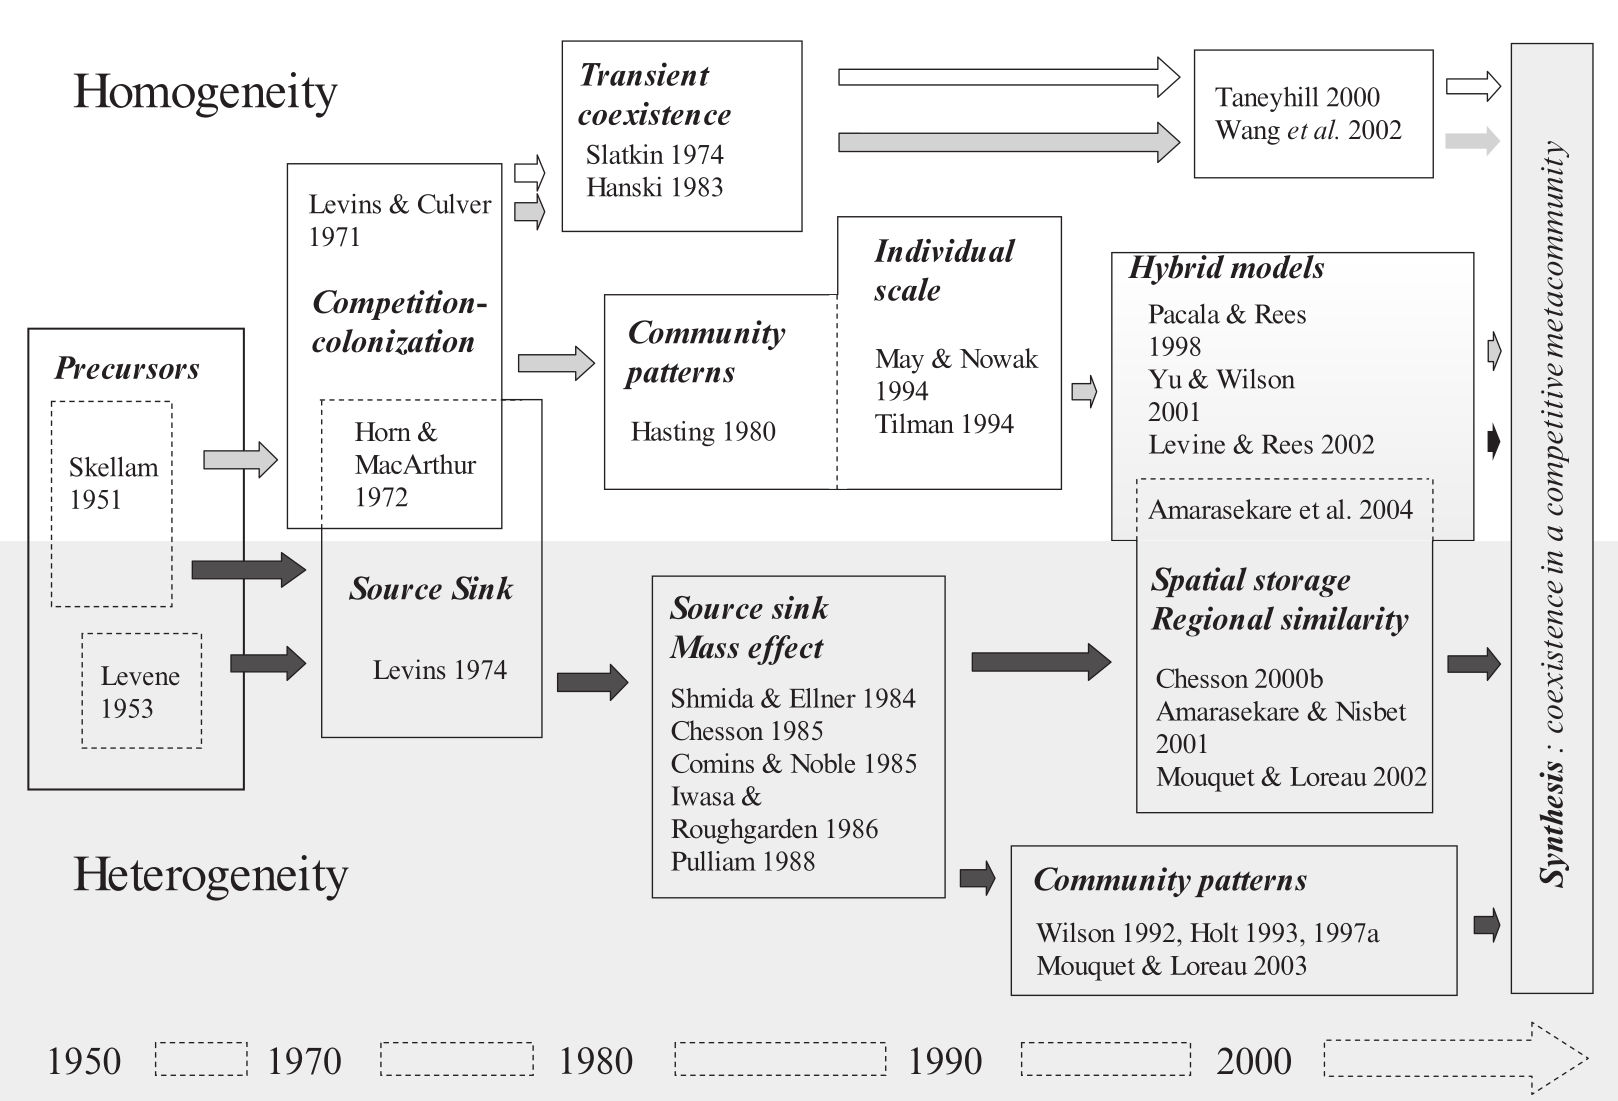
\includegraphics[height=0.7\textheight]{Figs/mouquet2005}\\
        \footnotesize Mouquet et al. 2005 in Holyoak et al. Metacommunity Ecology. Chicago University Press
    \end{center}

\end{frame}

%------------------------------
% HETEROGENEITY
%------------------------------

{
\usebackgroundtemplate{}
\begin{frame}

	\pagecolor{BDQC1st}
	\color{white}

	\LARGE{\textit{The world is patchy and heterogenous}}

\end{frame}
}

%------------------------------

{
\begin{frame}{The niche concept}

    \begin{center}
        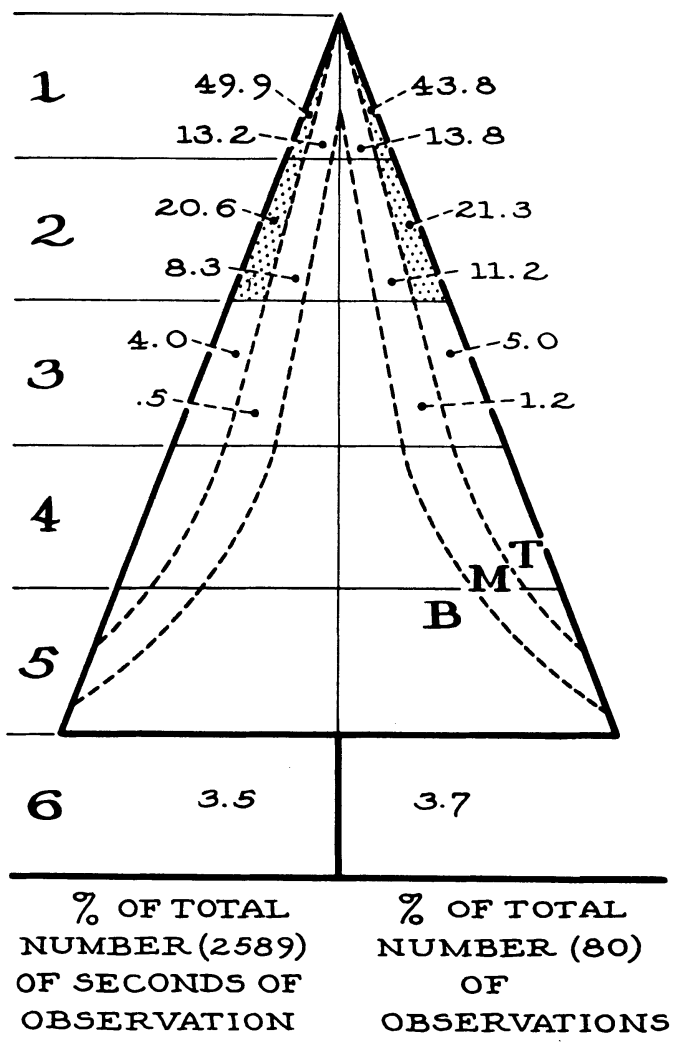
\includegraphics[height=0.7\textheight]{Figs/macarthur1958}\\
        \footnotesize MacArthur, R.H. 1958. Ecology
    \end{center}	

\end{frame}
}

%------------------------------

{
\begin{frame}{Species sorting}

    \begin{center}
        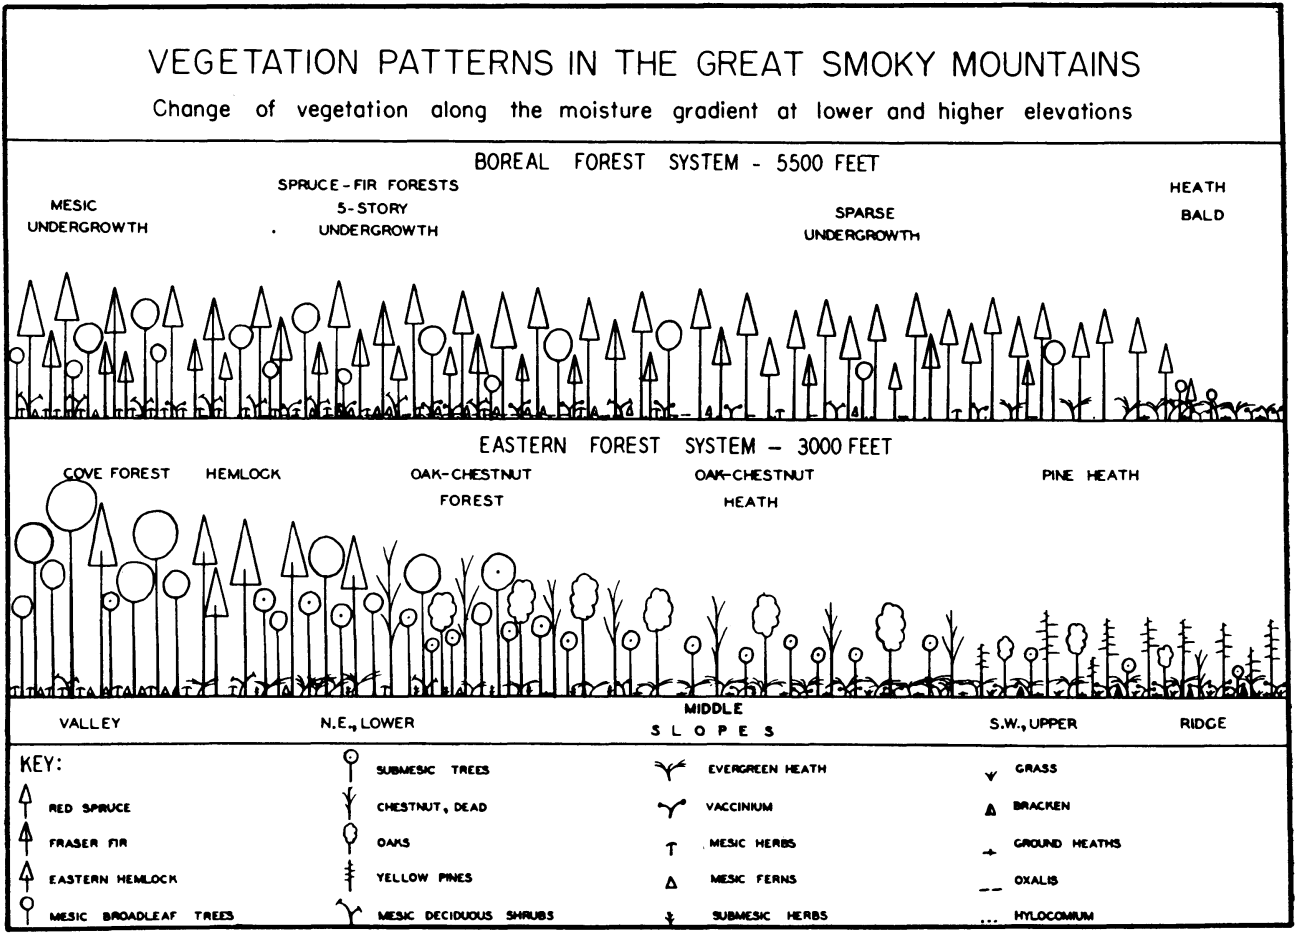
\includegraphics[height=0.6\textheight]{Figs/whittaker1956}\\
        \footnotesize Whittaker, R.H. 1956. Ecol. Monogr.
    \end{center}	

\end{frame}
}

%------------------------------

{
\begin{frame}{Disturbances}

    \begin{center}
        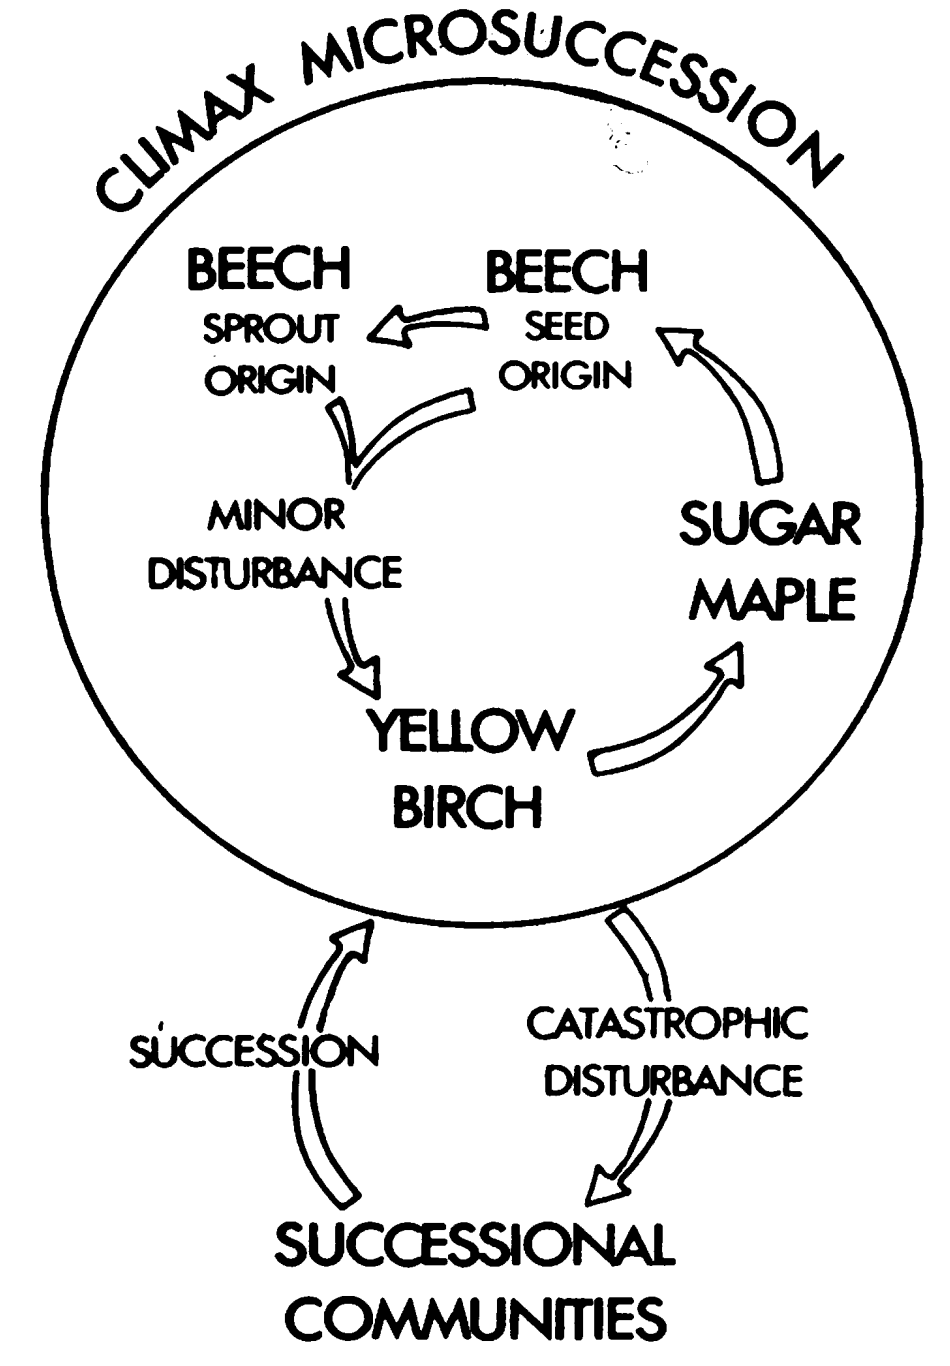
\includegraphics[height=0.7\textheight]{Figs/forcier1975}\\
        \footnotesize Clements, 1936; Tansley, 1935; Watt, 1947; (Forcier, 1975)
    \end{center}	

\end{frame}
}

%------------------------------
% LIMITED DISPERSAL
%------------------------------

{
\usebackgroundtemplate{}
\begin{frame}

	\pagecolor{BDQC1st}
	\color{white}

	\LARGE{\textit{Dispersal is limited}}

\end{frame}
}

%------------------------------

{
\begin{frame}{Diffusion theory}

    \begin{center}
        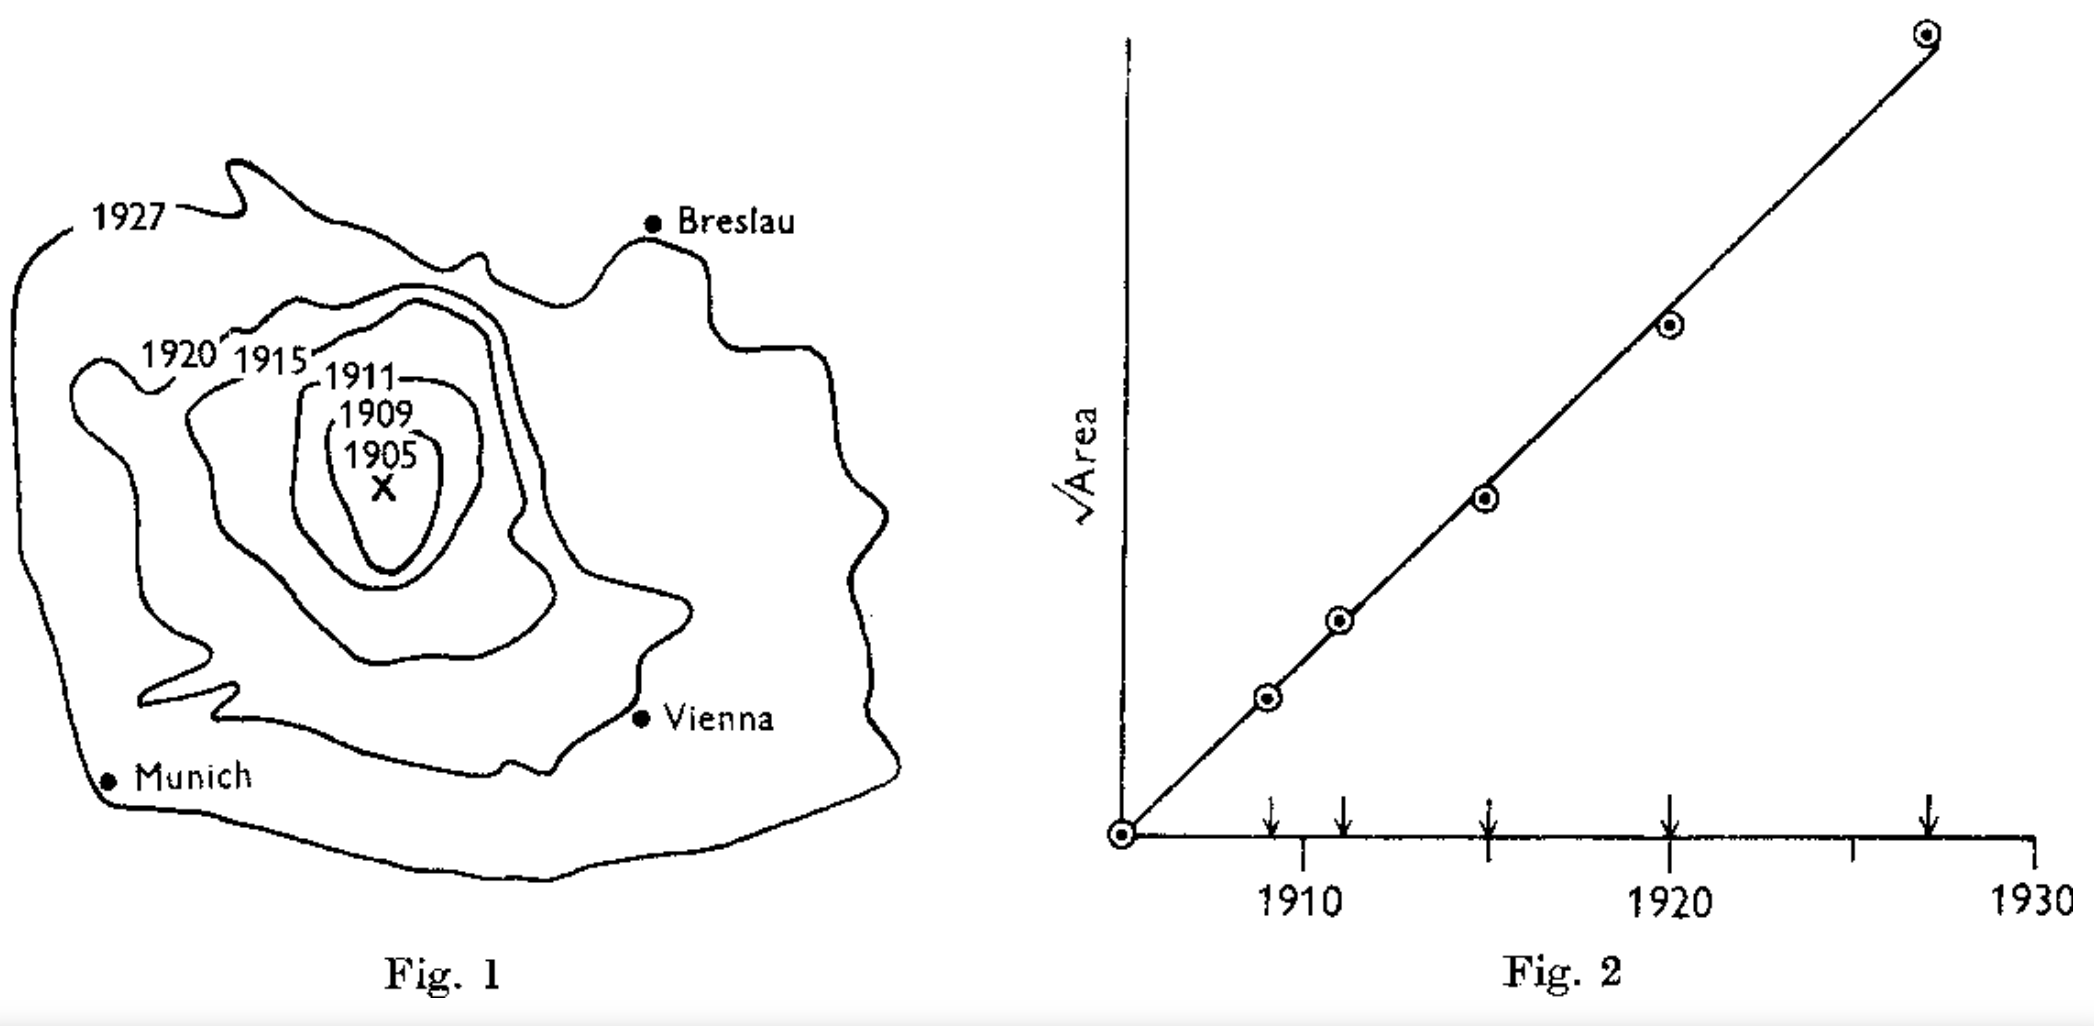
\includegraphics[height=0.7\textheight]{Figs/skellam1951}\\
        \footnotesize Skellam, J.G. 1951. Biometrika.
    \end{center}	

\end{frame}
}

%------------------------------

{
\begin{frame}{Patch occupancy}

    \begin{center}
        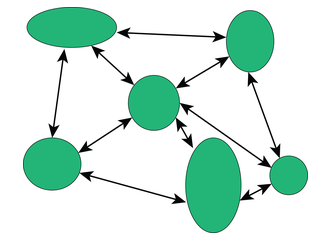
\includegraphics[height=0.7\textheight]{Figs/metapop}\\
        \footnotesize Levins, 1969. Bull. Entomo. Soc. Am.
    \end{center}	

\end{frame}
}

%------------------------------

{
\begin{frame}{Spatially explicit landscapes}

    \begin{center}
        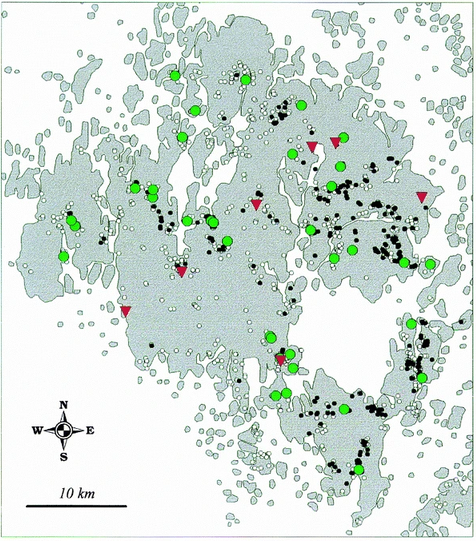
\includegraphics[height=0.7\textheight]{Figs/hanski1998}\\
        \footnotesize Hanski, I. 1994. J. Animal Ecol.
    \end{center}	

\end{frame}
}

%------------------------------

{
\begin{frame}{Patch formation}

    \begin{center}
        
\includegraphics[height=0.7\textheight]{Figs/rietkerk2004}\\
        \footnotesize Solé et al. 1992. Phys. Lett. A (Rietkerk et al. 2004)
    \end{center}	

\end{frame}
}

%------------------------------
% LOCAL-REGIONAL COUPLING
%------------------------------

{
\usebackgroundtemplate{}
\begin{frame}

	\pagecolor{BDQC1st}
	\color{white}

	\LARGE{\textit{Local-regional coupling contributes to diversity}}

\end{frame}
}

%------------------------------

{
\begin{frame}{Island biogeography}

    \begin{center}
        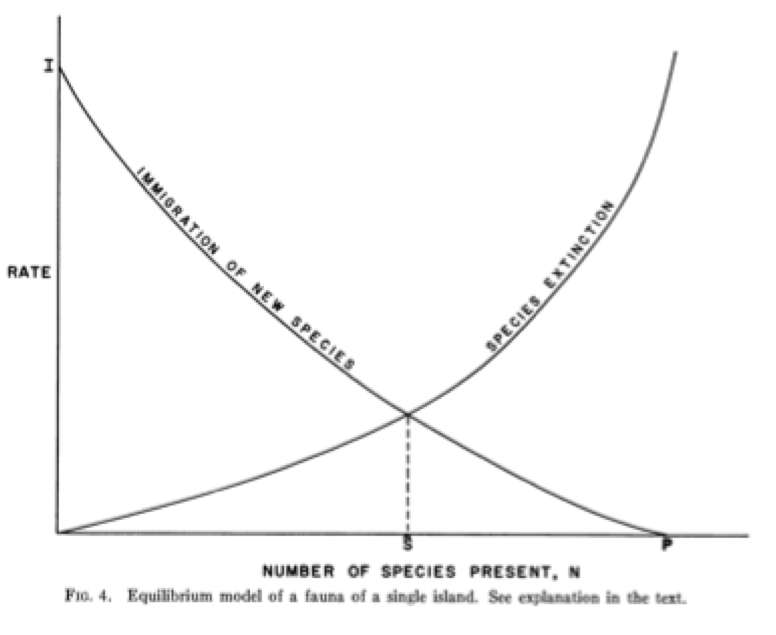
\includegraphics[height=0.7\textheight]{Figs/macarthur1963}\\
        \footnotesize MacArthur and WIlson. 1963. Evolution
    \end{center}	

\end{frame}
}

%------------------------------

{
\begin{frame}{Source-sink-dynamics}

    \begin{center}
        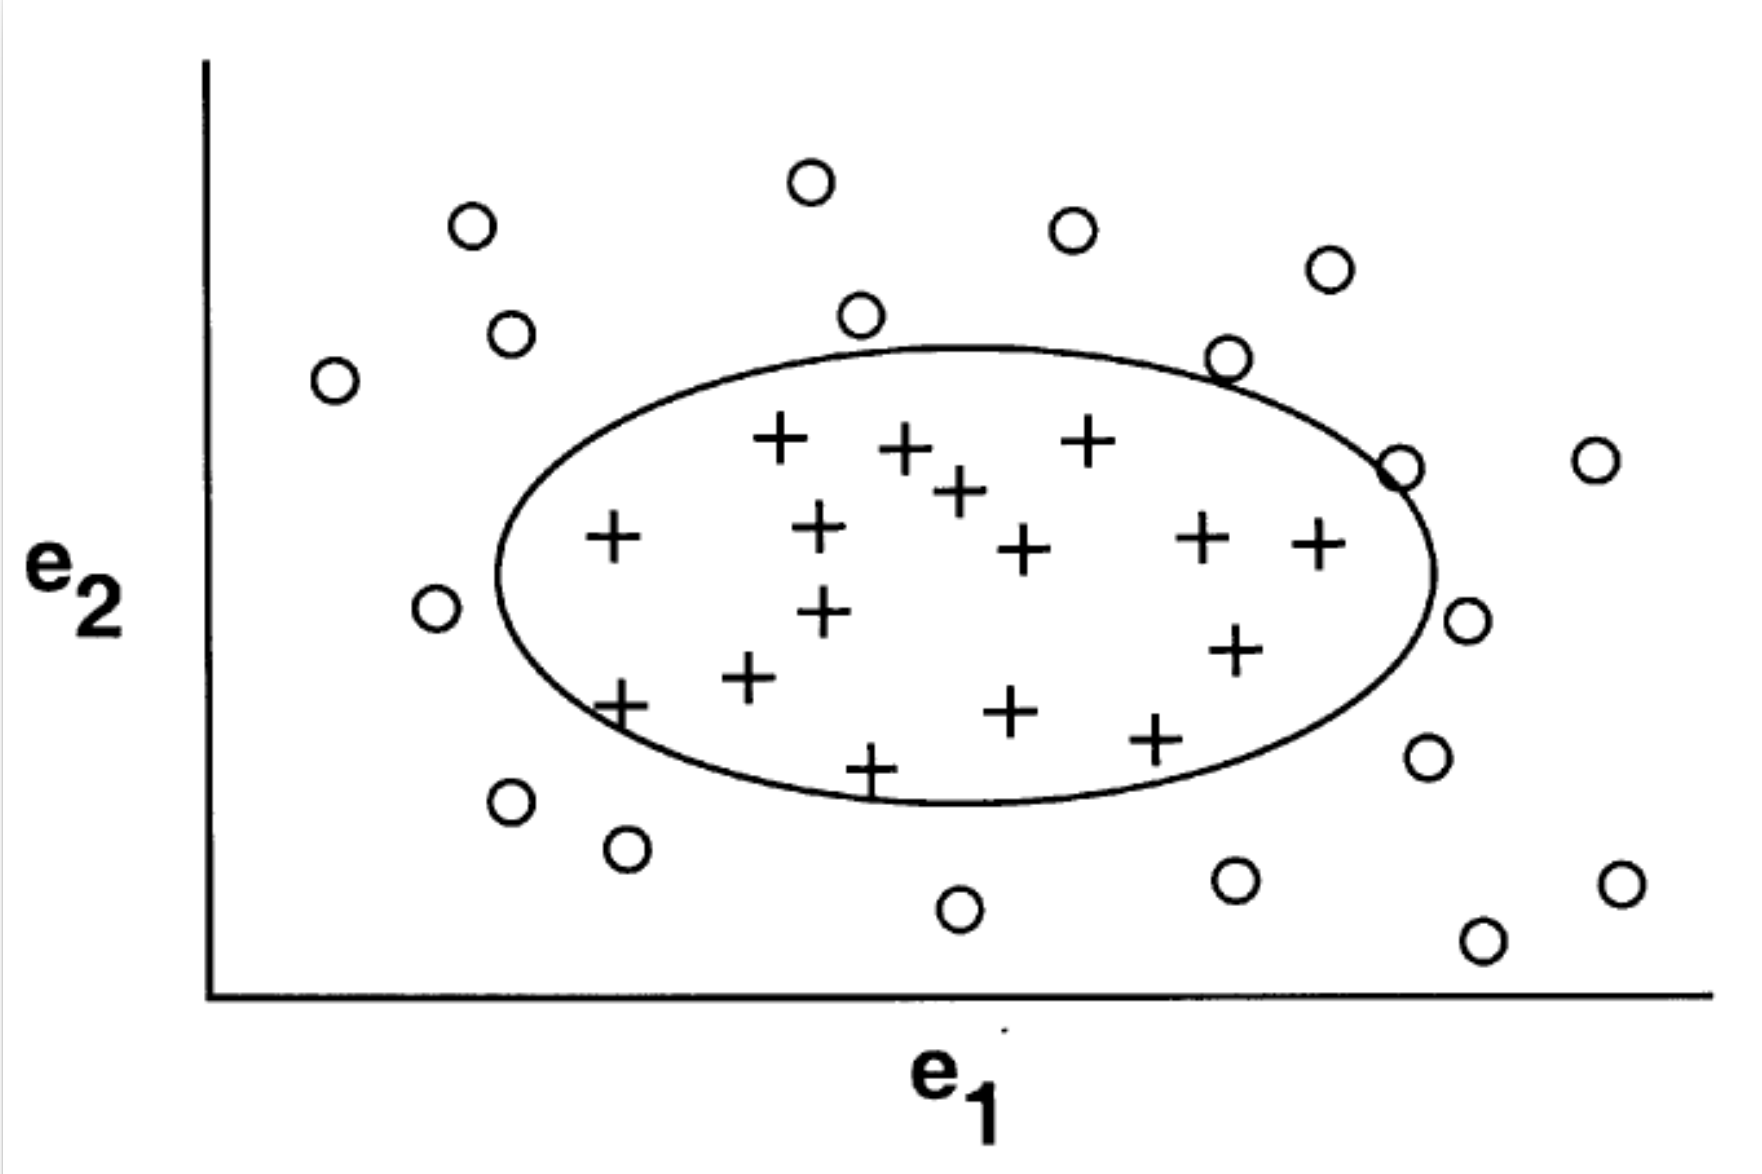
\includegraphics[height=0.7\textheight]{Figs/pulliam2000}\\
        \footnotesize Pulliam, R.H. 1988. Am. Nat.
    \end{center}	

\end{frame}
}

%------------------------------

{
\begin{frame}{Mass effect}

    \begin{center}
        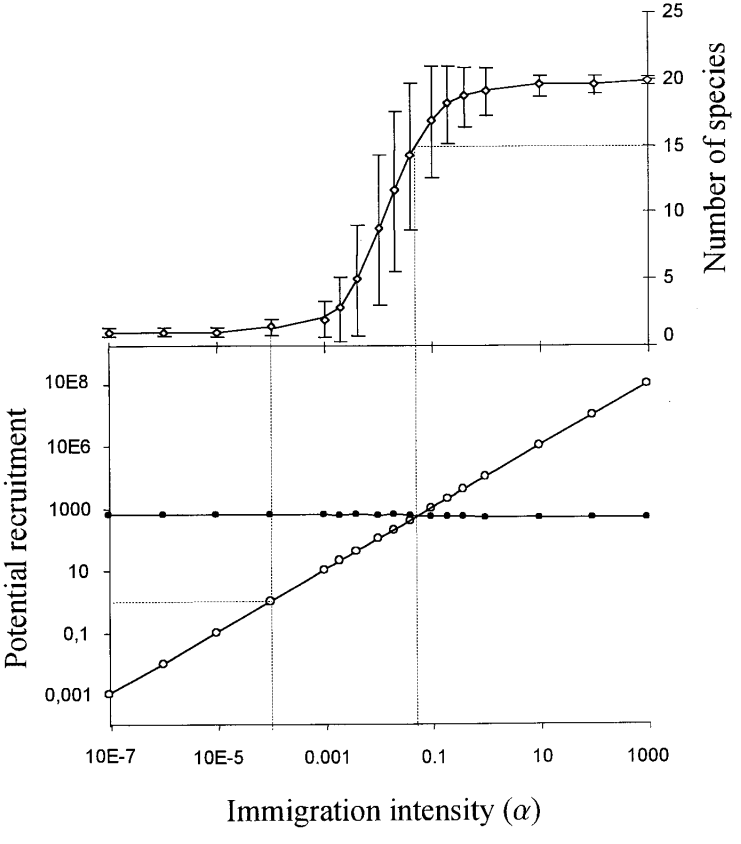
\includegraphics[height=0.7\textheight]{Figs/loreau1999}\\
        \footnotesize Loreau and Mouquet. 1999. Am. Nat.
    \end{center}	

\end{frame}
}

%------------------------------

{
\begin{frame}{Local-regional diversity relationship}

    \begin{center}
        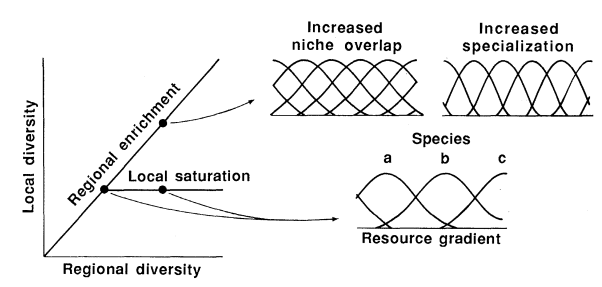
\includegraphics[height=0.7\textheight]{Figs/ricklefs1987}\\
        \footnotesize Ricklefs, R. 1987. Science.
    \end{center}	

\end{frame}
}

%------------------------------

{
\begin{frame}{Allochtonous inputs}

    \begin{center}
        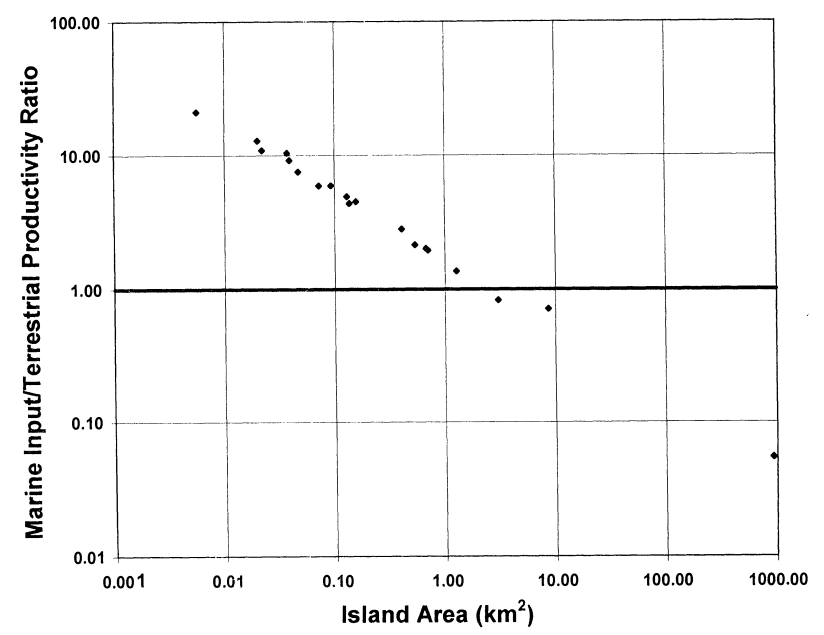
\includegraphics[height=0.7\textheight]{Figs/polis1996}\\
        \footnotesize Polis, G. et al. 1997. Ann. Rev. Ecol. Sys.
    \end{center}	

\end{frame}
}

%------------------------------
% Interaction with selection
%------------------------------

{
\usebackgroundtemplate{}
\begin{frame}

	\pagecolor{BDQC1st}
	\color{white}

	\LARGE{\textit{Heterogeneity, dispersal \& selection interact to impact community assembly}}

\end{frame}
}

%------------------------------

{
\begin{frame}{Arlequin dynamics and persistence}

    \begin{center}
        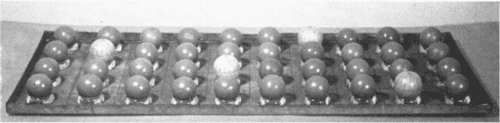
\includegraphics[height=0.4\textheight]{Figs/huffaker1958}\\
        \footnotesize Huffaker, C.B. 1958. Hilgardia.
    \end{center}	

\end{frame}
}

%------------------------------

{
\begin{frame}{Priority effects}

    \begin{center}
        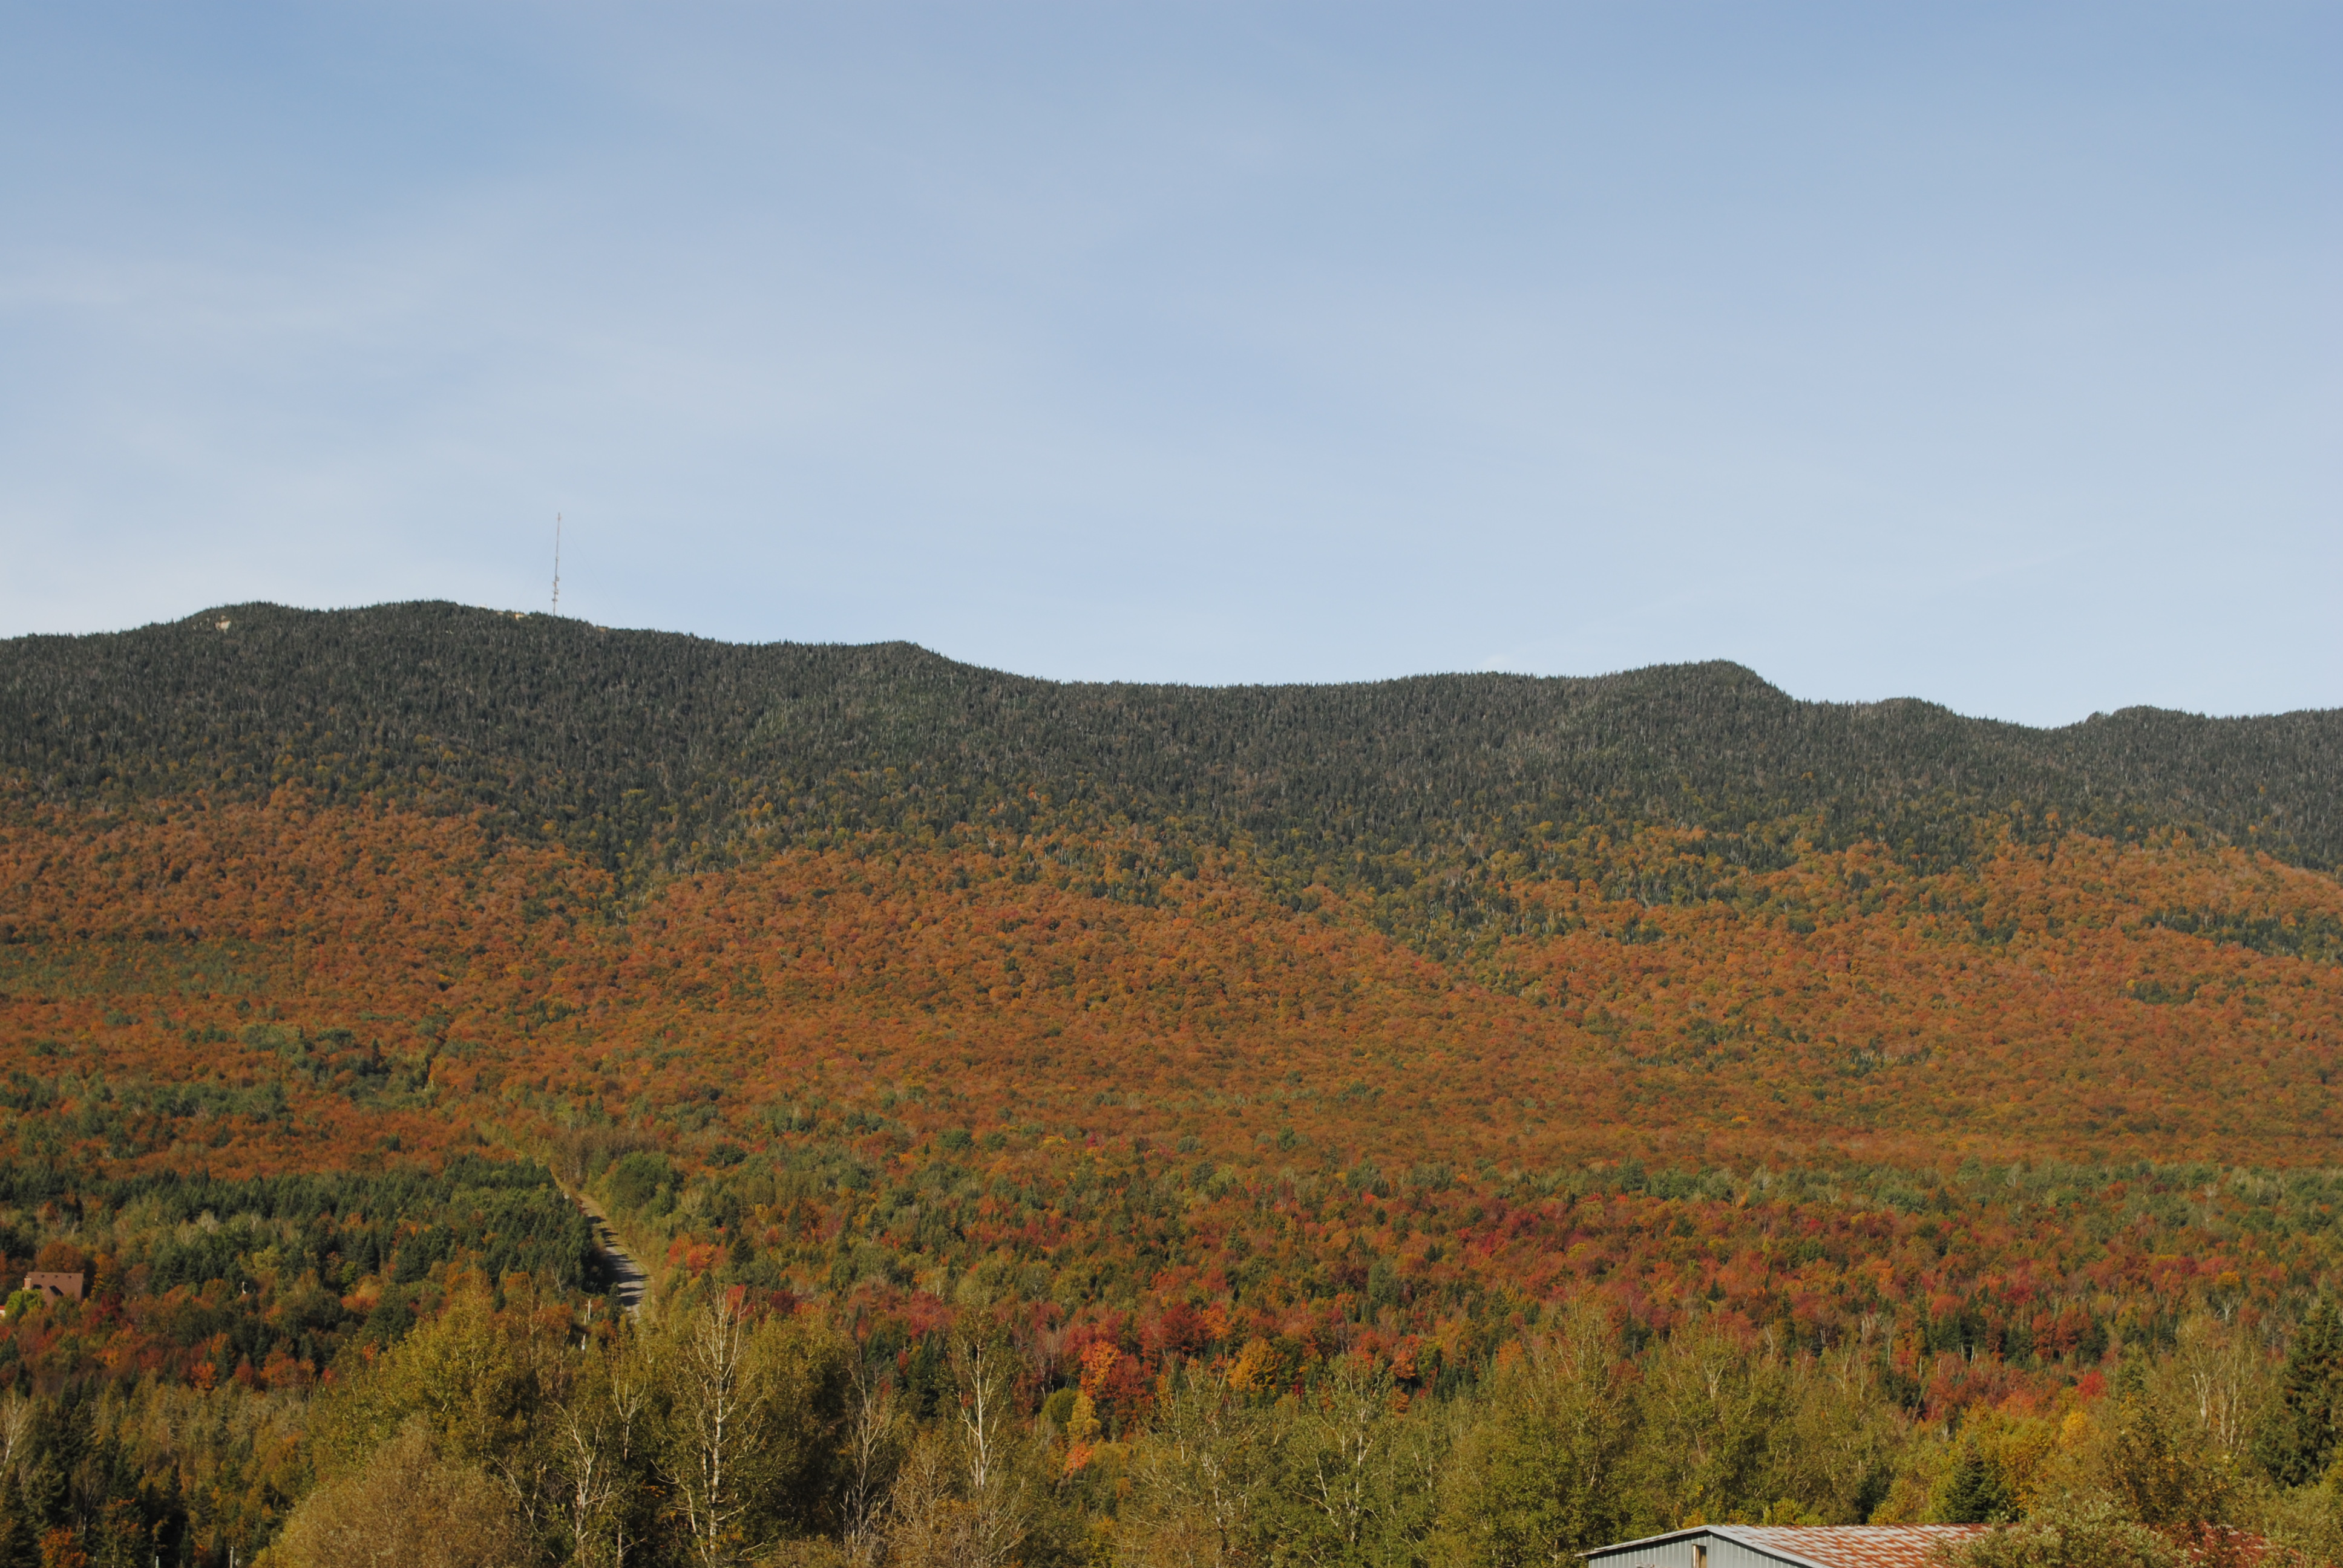
\includegraphics[height=0.7\textheight]{Figs/megantic}\\
        \footnotesize Hanski, I. 1983. Ecology.
    \end{center}	

\end{frame}
}

%------------------------------

{
\begin{frame}{Competition-colonization trade-off}

    \begin{center}
        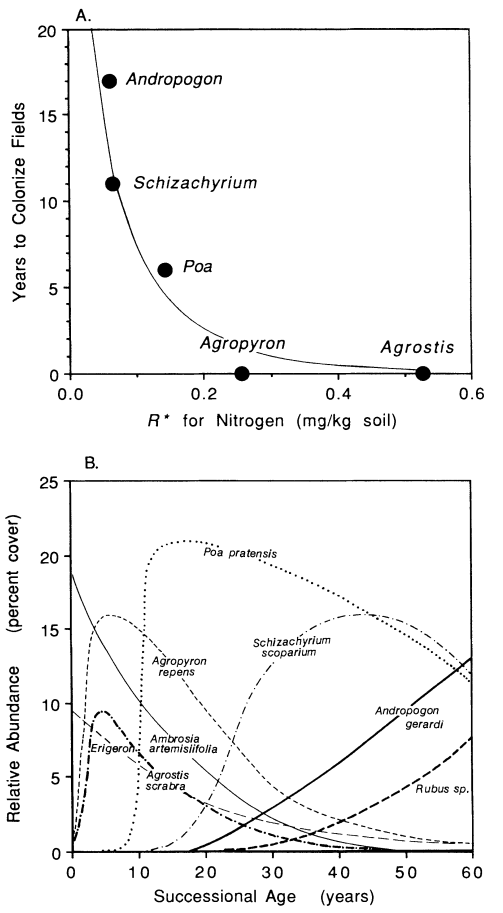
\includegraphics[height=0.7\textheight]{Figs/tilman1994}\\
        \footnotesize Hastins, 1980. Tilman, 1994.
    \end{center}	

\end{frame}
}

%------------------------------

{
\begin{frame}{Neutral theory}

    \begin{center}
        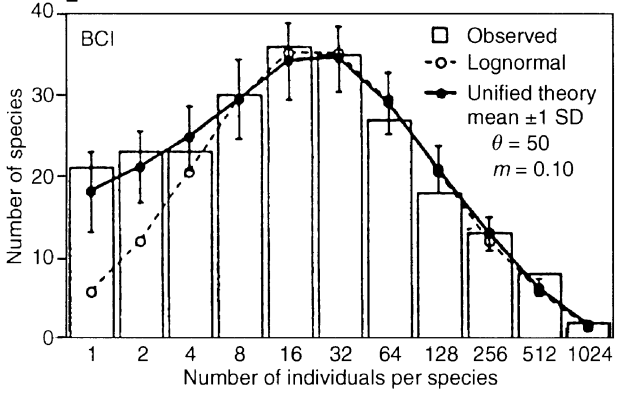
\includegraphics[height=0.7\textheight]{Figs/hubbell1997}\\
        \footnotesize Hubbell, 1997, 2001; Bell, 2000
    \end{center}	

\end{frame}
}

%------------------------------

{
\begin{frame}{Spatial inefficiency of predator-prey dynamics}

    \begin{center}
        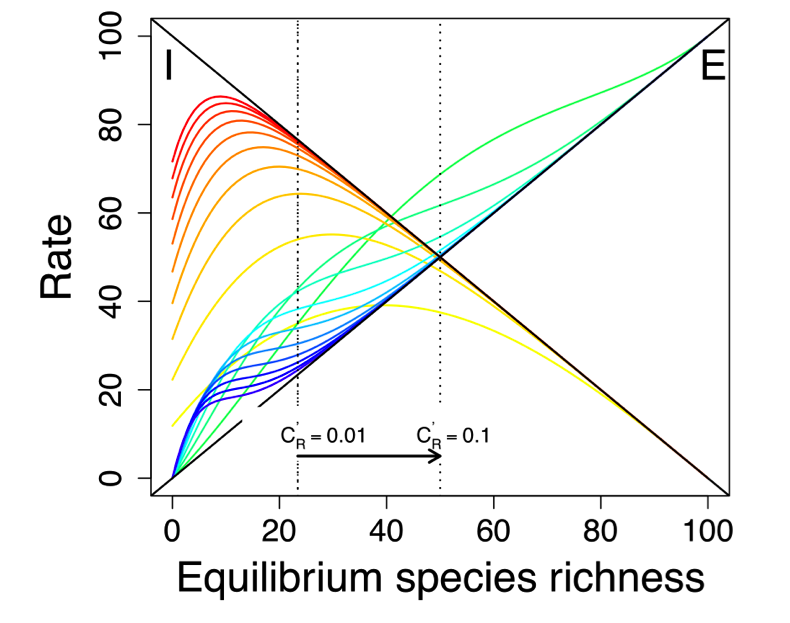
\includegraphics[height=0.7\textheight]{Figs/ttib}\\
        \footnotesize Holt et al. 1999. Ecology ; Gravel et al. 2011. Eco. Lett.
    \end{center}	

\end{frame}
}

%------------------------------

{
\begin{frame}{Spatial cascades}

    \begin{center}
        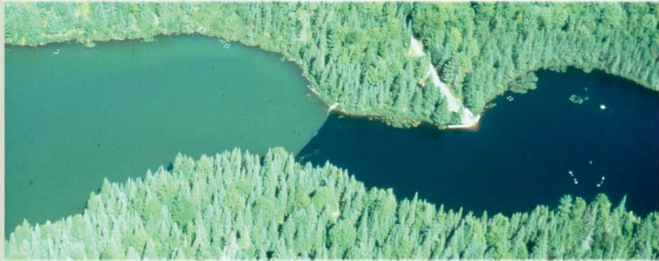
\includegraphics[height=0.5\textheight]{Figs/estes2011}\\
        \footnotesize Loreau et al. 2003, Eco. Lett.
    \end{center}	

\end{frame}
}

%------------------------------

{
\begin{frame}{Stability-complexity}

    \begin{center}
        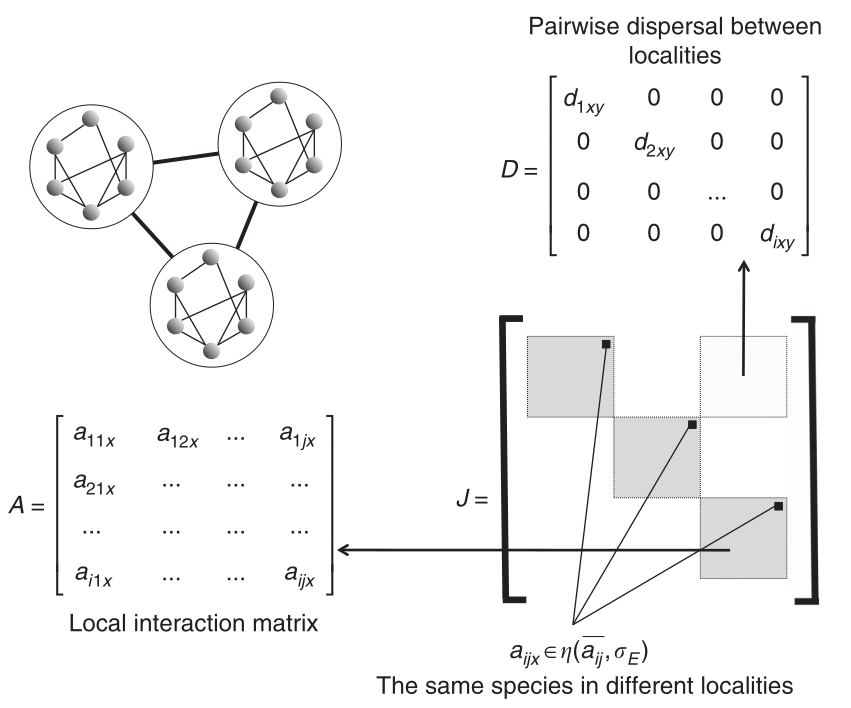
\includegraphics[height=0.7\textheight]{Figs/gravel2016}\\
        \footnotesize Gravel et al. 2016. Nat. Comm.
    \end{center}	

\end{frame}
}

%------------------------------

{
\begin{frame}{Distinct role of migration}

    \begin{center}
        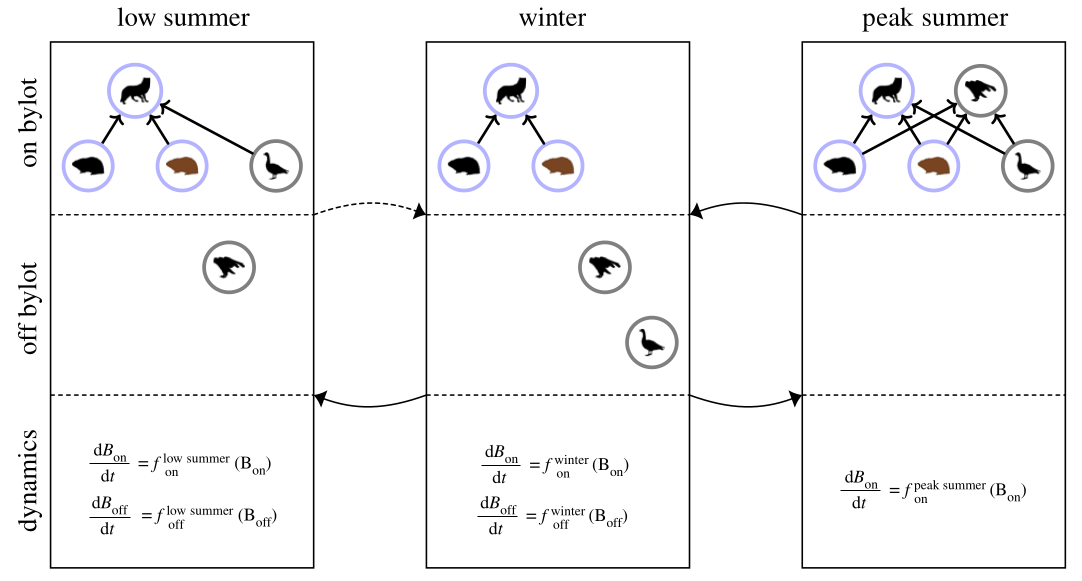
\includegraphics[height=0.7\textheight]{Figs/hutchison2020}\\
        \footnotesize Hutchison et al. 2020. Proc. Roy. Soc. London A
    \end{center}	

\end{frame}
}

%------------------------------

{
\begin{frame}{Moments of metacommunities}

    \begin{center}
        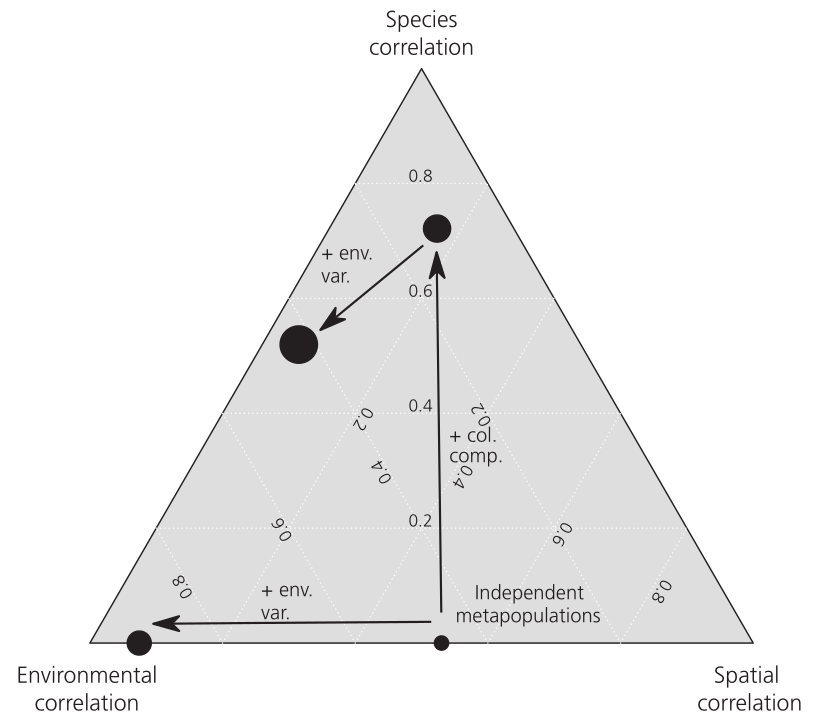
\includegraphics[height=0.7\textheight]{Figs/gravel2020}\\
        \footnotesize Gravel and Massol. 2020 in McCann et al. Theoretical Ecology. Oxford University Press.
    \end{center}	

\end{frame}
}


%------------------------------
% CONCLUSION
%------------------------------

{
\usebackgroundtemplate{}
\begin{frame}

	\pagecolor{BDQC1st}
	\color{white}

	\LARGE{\textit{Spatial ecology in the context \\ of global changes ?}}

\end{frame}
}

%------------------------------

%------------------------------
%------------------------------
%------------------------------
%------------------------------
\end{document}
